%_____________________________________________________________________________________________ 
% LATEX Template: Department of Comp/IT BTech Project Reports
% Sample Chapter
% Sun Mar 27 10:25:35 IST 2011
%
% Note: Itemization, enumeration and other things not shown. A sample figure is included.
%_____________________________________________________________________________________________ 

\chapter{Introduction}

\section{Importance of Automatic Question Generation (AGS) Systems}

Gauging a student’s knowledge over a certain topic is one of the fundamental
problems in education systems. Quizzing students has long been accepted as one
of the best techniques to solve the problem. Studies conducted over the last
several decades have found that providing students with frequent and good number
of quiz questions leads to better understanding of the topics, than spending an
equal amount of time studying notes or textbooks. Quizzes can be used at several
places in the education domain. It can be used in MOOC’s to test if a student
has  grasped the concept properly, they can be used as standalone tests in
universities, or they can also be used as practice by students to discern their
command over the subject. 

However, with the volume of information available, generating questions from
domain experts is an expensive and time consuming process. The task of Automatic
Question Generation (AQG), in the field of Natural Language Processing, aims to
generate questions from a given text, such that students are appropriately
tested on their mastery over the subject.

\section{Neural Networks}

A neural network is an interconnected collections of neurons. The connections
between the neurons are modelled as weights and the final value that the neuron
stores is the weighted summation of all the inputs. A neural network consists of
an input layer, an output layer and multiple hidden layers.

\begin{figure}
	\caption{Basic Neural Network Diagram}
	\centering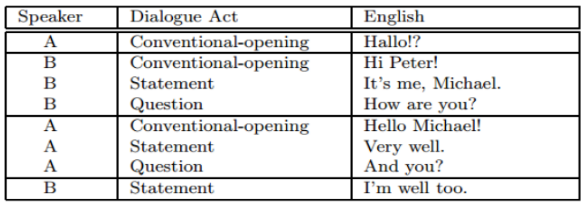
\includegraphics[width=10cm]{1.png}
\end{figure}

\section{Recurrent Neural Networks (RNN)}

Recurrent neural network is a type of artificial neural network. The problem of
remembering previous inputs to the network was solved by recurrent neural
networks with the help of hidden layers. Because of their internal memory, RNN
is able to remember important things about the input, which allows them to make
precise predictions about what’s coming next. This is why they are preferred
algorithm for sequential data. Sequential data is just ordered data where
related things follow each other.

\begin{figure}
	\caption{Recurrent vs Feed-forward Neural Network}
	\centering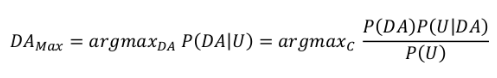
\includegraphics[width=10cm]{2.png}
\end{figure}

Unlike the normal feedforward neural networks, recurrent neural networks feed
the output of previous step to the current step. This helps the network to
memorise the previous inputs. So basically RNN cycles through the information,
i.e. when taking a decision it takes into consideration the current input as
well as whatever it learned from the previous output. For example, consider the
word ‘Teacher’, till the point a feed forward neural network reaches ‘c’ it
forgets about ‘t’, ‘e’ and ‘a’. A RNN remembers exactly that. Recurrent Neural
Network adds immediate past to the present. This is important since past data
contains information about what is coming next. 

RNN applies weight to current and also previous input and they tweak their
weights through gradient descent and backpropagation through time. Gradient
Descent is an algorithm that is used to iteratively minimize a given function.
Backpropagation Through Time (BPTT) is basically just a fancy buzz word for
doing Backpropagation on an unrolled Recurrent Neural Network. Unrolling is a
visualization and conceptual tool, which helps you to understand what’s going on
within the network. RNN can be viewed as a sequence of Neural Networks that is
trained one after another with backpropagation.

\begin{figure}
	\caption{Structure of a Neuron}
	\centering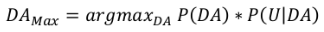
\includegraphics[width=10cm]{3.png}
\end{figure}

The above diagram shows the RNN being unrolled after the equal sign. The
different timesteps are visualized and information gets passed from one timestep
to the next. Within BPTT the error is back-propagated from the last to the first
timestep, while unrolling all the timesteps. This allows calculating the error
for each timestep, which allows updating the weights.

\subsection{Problems with RNN}

\begin{enumerate}[align=left]

	\item Training RNNs is a difficult task.

	\item \textbf{Exploding gradient problem :} Exploding gradient is when
		the algorithm assigns a stupidly high importance to the weights,
		without much reason. But fortunately, this problem can be easily
		solved if you truncate or squash the gradients.

	\item \textbf{Vanishing gradient problem :} Vanishing gradient is when
		the values of a gradient are too small and the model stops
		learning or takes way too long because of that. This problem is
		solved by the concept of LSTM.

\end{enumerate}

\section{Long Short Term Memory}

Long Short Term Memory (LSTM) is an artificial recurrent neural network.
Consider LSTM as an extension to the recurrent neural network, which basically
extends its memory. Therefore they are capable of learning things that have very
large time lags between them. LSTM can remember this because they contain their
information in a memory, that is much like the memory of a computer because the
LSTM can read, write and delete information from its memory.

The memory in LSTM are gated cells. Gated cell means that he cell decides
whether or not to store or delete information based on the importance it assigns
to the information. The importance assigning takes place through weights which
are learned through the algorithm.

\begin{figure}
	\caption{Structure of a Basic LSTM node}
	\centering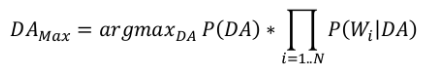
\includegraphics[width=10cm]{4.png}
\end{figure}

A basic LSTM node consists of input gate, output gate and forget gate. The input
gate decides whether or not to let new input in. The forget gate deletes the
information because it is not important. The output gate impacts the output at
the current time step. The gates in a LSTM are analog, in the form of sigmoids,
meaning that they range from 0 to 1. The fact that they are analog, enables them
to do backpropagation with it.

The problem of vanishing gradients which is very common in recurrent neural
networks is solved by LSTM as it keeps the gradient steep enough and therefore
the training short and the accuracy high.
